\section{Convolutional Codes}
\subsection{TCM - Trellis Coded Modulation}
\subsubsection{Convolutional Coding - Faltungs Code}
Ein Faltungs Code besitzt zur Logikschaltung zus\"atzlich noch Memory, so dass
nicht nur der aktuelle Eingang sondern auch noch $n$-vorherige Eing\"ange zum
Ausgang verrechnet werden. Es gibt m unterschiedliche Ausg\"ange. 
Je nach Vorgeschichte, k\"onnen nur noch ganz bestimmte Kombinationen auftreten,
was dann die Decodierung besser macht.\\
\begin{minipage}{9cm}
	Beispiel mit k=1; n=2; m=2 $\to$ 1/2 codierung\\
	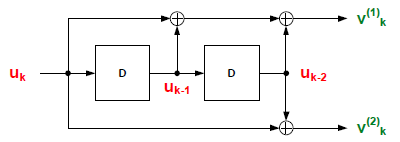
\includegraphics[width=9cm]{./bilder/covolutionSchemata.png}
\end{minipage}
\hspace{5mm}
\begin{minipage}{8cm}
\vspace{4mm}
	mit dazugeh\"origem Encoder State Diagram\\
\hspace{5mm}
	\includegraphics[width=6cm]{./bilder/covolutionStateDiagram.png}
\end{minipage}
\\
\textbf{Generator Sequences}\\
Die Generatorsequenzen erhält man dadurch, dass eine einzelne Eins (...000000100000...) an 
den Eingang gegeben wird. Somit lauten die Generatorsequenzen für obiges Blockdiagram:\\
$g^{(1)}=(1 1 1)$ resp. $g^{(2)}=(1 0 1)$

\subsubsection{Decodierung}
Eine gute Variante die FaltungsCodes zu dekodieren ist dies mit einem Trellis
Diagram zu machen: \\
\begin{minipage}{10cm}
	\begin{liste}
		\item Zuerst Punkte entsprechend der m\"oglichen Speicherinhalte einzeichnen.
		\item M\"ogliche Verbindungen einzeichnen.
		\item Sollwerte einzeichnen (z.B. 0/00).
		\item Fehler zu den einzelnen Punkten eintragen (ev. die Euklidische Distanz). Wird auch Zustandsmetrik genannt.
		\item Wenn zwei Wege zu einem Punkt kommen, den h\"oherwertigen Weg streichen.
		\item Am Schluss den Weg nehmen der den kleinsten Fehler ergibt.
	\end{liste}
\end{minipage}
\begin{minipage}{9cm}
	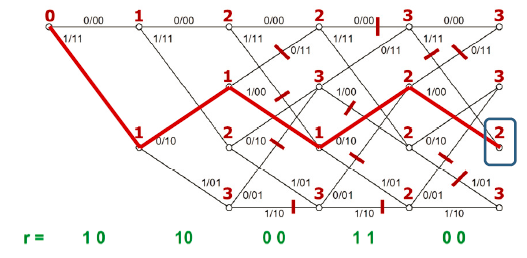
\includegraphics[width=9cm]{./bilder/Trelli.png}
\end{minipage}\\
\textbf{Soft Decoding}\\
Im Falle von Soft Decoding, liefert  der Demodulator eine reelle Zahl zwischen 0 und 1. Mit der quadrierten 
eklidischen Distanz kann man dann die Zustandsmetriken wie folgt berechnen: \\
$M_{000}[k]=min(M_{000}[k-1]+(r_1[k]-v_1[k])^2+(r_2[k]-v_2[k])^2; M_{001}[k-1]+(r_1[k]-v_1[k])^2+(r_2[k]-v_2[k])^2)$ \\
Beispiel:\\
$M_{000}[k-1]=3.5$ und $M_{001}[k-1]=3.0$ und $r_1[k]=0.5$ und $r_2[k]=0.9$\\
Angenommen der Zustand bei $[k-1]$ war $M_{000}$, dann ist der Zustandübergang 0/00. Falls der Zustandswechsel 
hingegen von $M_{001}$ kommt, dann ist der Zustandsübergang 0/11. Somit ergibt sich:\\
$M_{000}[k]=min(3.5+(0.5-0)^2+(0.9-0)^2; 3.0+(0.5-1)^2+(0.9-1)^2)=min(4.56; 3.26)=3.26$ \\



\subsubsection{Euklidische Distanz}
\begin{minipage}{13cm}
	Die \textbf{euklidische Distanz} ist der Abstand zwischen zwei
	unterschiedlichen Modulationspositionen.\\
	Die \textbf{freie euklidische Distanz} ist der minimale Abstand zwischen zwei
	unterschiedlichen Modulationspositionen in der ganzen Modulation.\\
	$d^2_{free}=\min \limits_{a_k \neq a_{k}^{'}} \sum \limits_k
	d^2(a_k,a_{k}^{'})$\\
	zB.	$d^2_{min}=1 + 1 -2\cos (\alpha)= 2-\sqrt{2} = 0.586$\\
	Der \textbf{Coding Gain} ist um welchen Faktor der SNR schlechter sein darf.\\
	$G = \frac{d^2_{free,coded}}{d^2_{min, uncoded}}$
\end{minipage}
\begin{minipage}{6cm}
	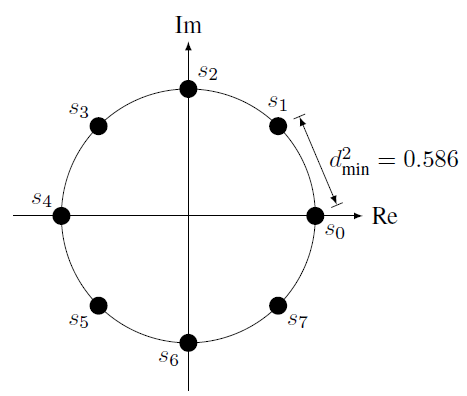
\includegraphics[width=6cm]{./bilder/EuklidischeDistanz.png}
\end{minipage}